\chapter{Resultados y conclusiones}\label{chap:part1conclusions}

Para poder valorar la utilidad real de la aplicación frente a los distintos
dispositivos ya disponibles y que realizan una función semejante se ha
decidido comparar los resultados que se obtienen al utilizar la tarjeta y
un osciloscopio, como elemento representativo, en una prueba genérica.

Por separado, se ha evaluado el rendimiento de subsistema de interacción
con el medio físico (el conjunto formado por los circuitos acondicionadores
y los transductores de ultrasonidos).


\section{Prueba comparativa}\label{sec:working-test}

La prueba realizada es muy sencilla y sirve para valorar la operatividad de
la aplicación y sus límites. Consiste en conectar la sonda de un
osciloscopio y unas sondas con conectores tipo <<banana>> adaptados para
trabajar con la caja de conexiones (\vref{fig:conbox}) a un generador de
señales y comparar los resultados que se obtienen con cada uno de los
dispositivos.

La metodología de la prueba es la siguiente: para los distintos tipos de
señal que genera un generador de señales, se modifican la frecuencia y la
amplitud de la señal y se comparan los resultados obtenidos con la
aplicación y los resultados obtenidos con el osciloscopio. Adicionalmente
se comprueba que el resto de funciones de la aplicación proporcionen los
resultados esperados.

La \cref{tab:testparameters} muestra los tipos de señales y los valores de
los parámetros utilizados durante la realización de las pruebas. Las
funciones de la aplicación cuyo comportamiento se observa son las listadas
a continuación:

\begin{itemize}
    \item Selección de canal. Para cada canal/puerto de entrada se ha
	evaluado la respuesta en presencia y ausencia de señal, en el
	puerto activo y en el resto.
    \item Ajustes de ganancia, modo de adquisición y frecuencia (sólo para
	medidas numéricas).
    \item Se ha evaluado el funcionamiento de los tres modos de medición
	(medidas numéricas y representación gráfica).
    \item En el modo gráfico de funcionamiento:
	\begin{itemize}
	    \item Ajuste de la escala temporal/horizontal y repercusión en
		la elección del modo de representación. Se han evaluado los
		resultados obtenidos al seleccionar cada uno de los modos.
	    \item Funcionamiento de los controles de las ventanas de
		representación, tanto de los que alteran la escala de
		amplitud/vertical como el que permite alternar la ventana
		en la que son representadas la señal y su espectro.
	    \item Ajuste del número de puntos para el cálculo de la
		\sig{fft}.
	\end{itemize}
\end{itemize}

\begin{table}
    \centering
    \begin{tabular}{l d{5.1}d{8.1}d{2.1}}
	\toprule
	& \multicolumn{3}{c}{Parámetros de la señal} \\
	\cmidrule(l){2-4}
	Tipo de señal & \multicolumn{1}{c}{Frecuencia (Hz)} &
	    \multicolumn{1}{c}{Periodo ($\mu\text{s}$)} &
	    \multicolumn{1}{c}{Amplitud ($\text{V}_\text{pp}$)} \\
	\midrule
		    & 0,1	& 10000000	& \\
		    & 1		& 1000000	& \\
	Sinusoidal  & 5		& 2000000	& 16 \\
		    & 25	& 40000		& \\
	Rectangular & 1000	& 10000		& 10 \\
		    & 1000	& 10000		& \\
	Triangular  & 10000	& 100		& 1 \\
		    & 20000	& 50		& \\
	Pulsada	    & 30000	& 33,3		& 0,1 \\
		    & 40000	& 25		& \\
		    & 50000	& 20		& \\
	\bottomrule
    \end{tabular}
    \caption[Parámetros de la prueba]{Parámetros de la prueba.}
    \label{tab:testparameters}
\end{table}

Dada la multitud de variables que intervienen en la realización de las
pruebas se obtiene una gran cantidad de resultados, en este documento se ha
optado por ofrecer sólo una muestra de los resultados así como las
conclusiones que se infieren a la vista de los mismos.


\subsection{Resultados de las pruebas}

A continuación se expone una batería de imágenes que representan los
distintos resultados obtenidos al someter la aplicación a las pruebas
descritas utilizando los siguientes parámetros: señal sinusoidal,
frecuencia de 5 kHz, y amplitud de 16 $\text{V}_\text{pp}$. Se ha observado
el funcionamiento de la representación gráfica al seleccionar distintos
valores de escala temporal y número de puntos para la realización de la
\sig{fft}. También se ha verificado el funcionamiento de los controles que
habilitan/deshabilitan la representación de la señal o de su espectro en
frecuencia, y permiten alternar la ventana en la que se hace cada
representación.

\begin{figure}
    \begin{center}
	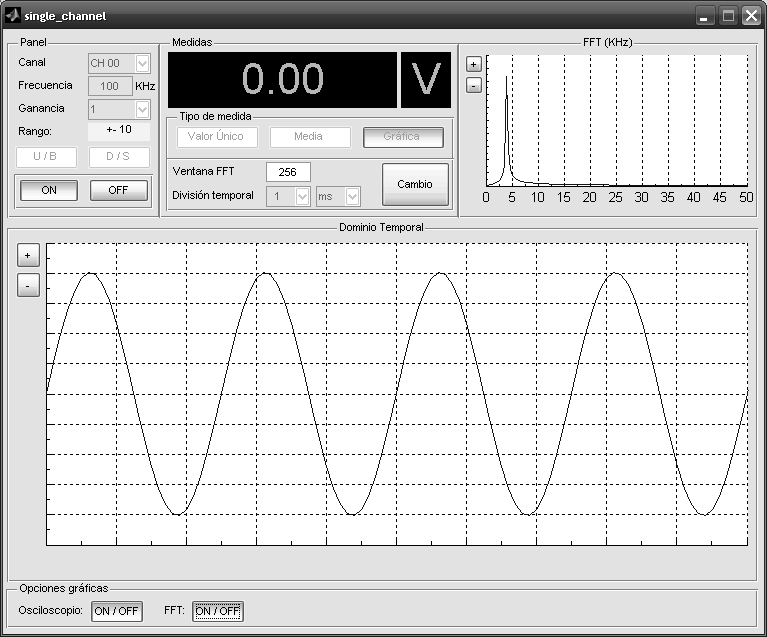
\includegraphics{gis-pfc-ch4-01.png}
    \end{center}
    \caption[Representaciones obtenidas utilizando diversas
    configuraciones]{Representación de los datos utilizando la
    configuración por defecto.}
    \label{fig:test1}
\end{figure}

\begin{figure}\ContinuedFloat
    \begin{center}
	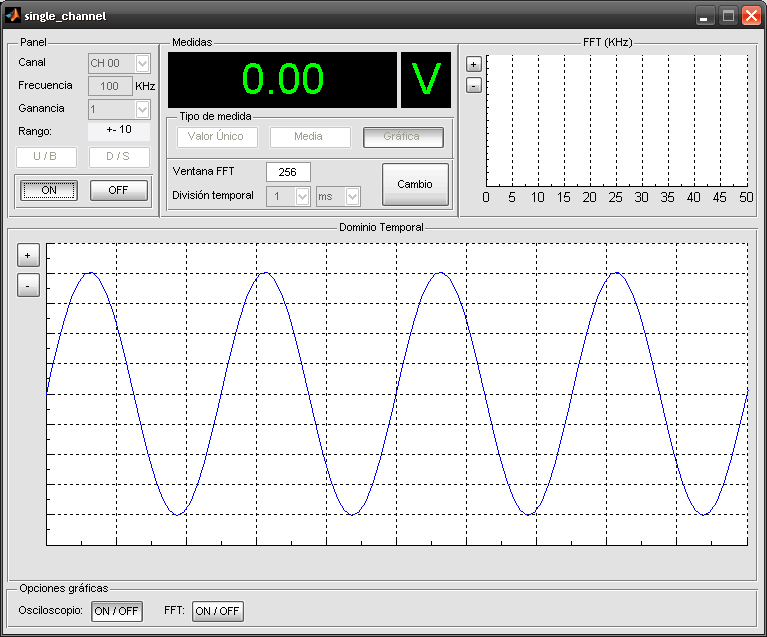
\includegraphics{gis-pfc-ch4-02.png}
    \end{center}
    \caption[]{Representación únicamente de la señal, representación del
    espectro deshabilitada.}
    \label{fig:test2}
\end{figure}

\begin{figure}\ContinuedFloat
    \begin{center}
	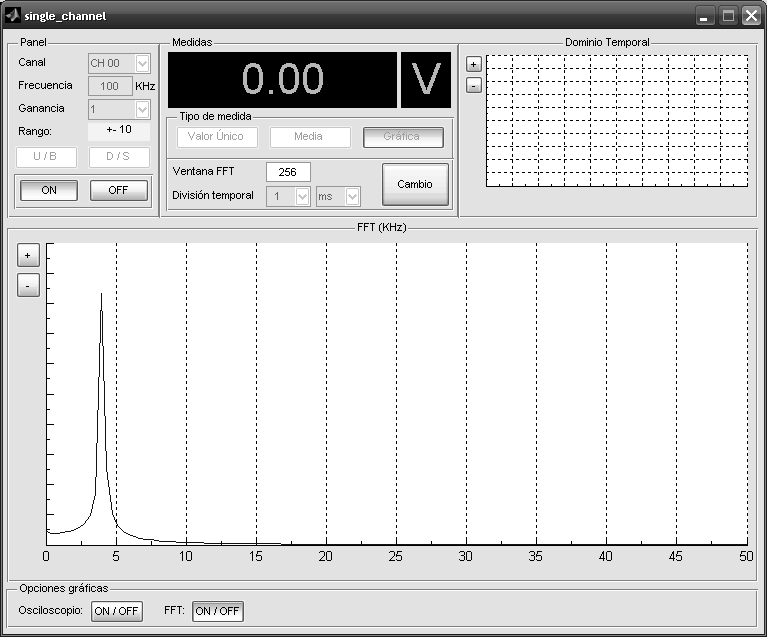
\includegraphics{gis-pfc-ch4-03.png}
    \end{center}
    \caption[]{Representación únicamente del espectro (en la ventana
    principal), representación de la señal deshabilitada.}
    \label{fig:test3}
\end{figure}

\begin{figure}\ContinuedFloat
    \begin{center}
	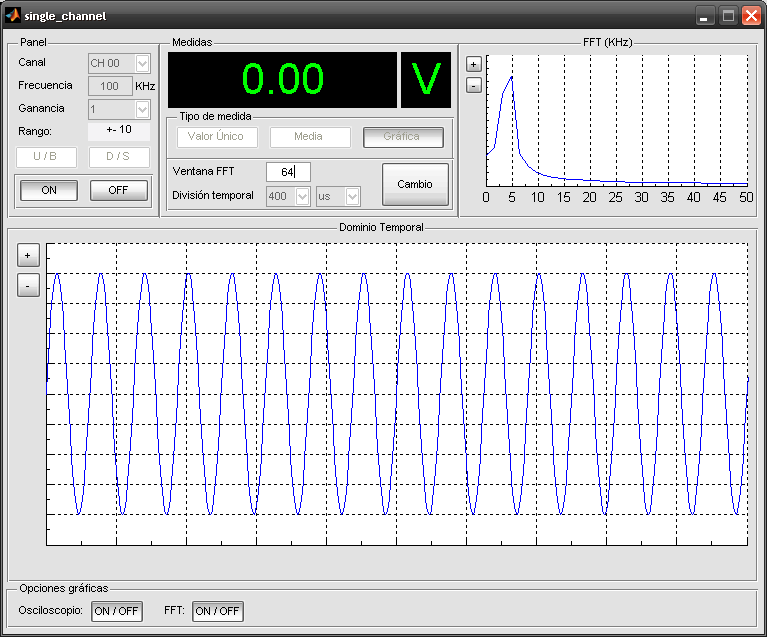
\includegraphics{gis-pfc-ch4-04.png}
    \end{center}
    \caption[]{Representación de la señal utilizando una escala temporal
    distinta a la escala por defecto, duración de la señal representada de
    4ms ---frente a los 10 ms por defecto---. La \sig{fft} se ha calculado
    con un número menor de puntos, 64 ---la cuarta parte del número por
    defecto 256---.}
    \label{fig:test4}
\end{figure}

\begin{figure}\ContinuedFloat
    \begin{center}
	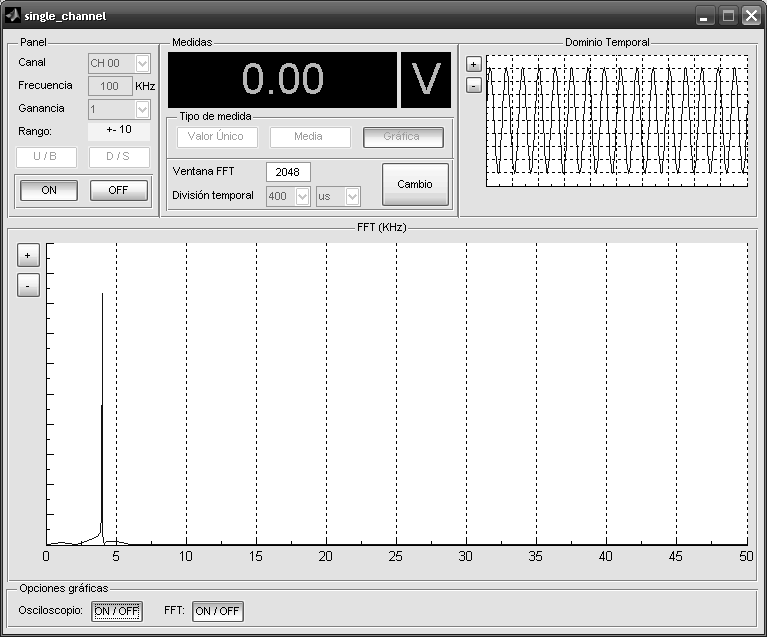
\includegraphics{gis-pfc-ch4-05.png}
    \end{center}
    \caption[]{Representación del espectro utilizando para ello la
    \sig{fft} calculada con una mayor cantidad de puntos (2048).}
    \label{fig:test5}
\end{figure}
